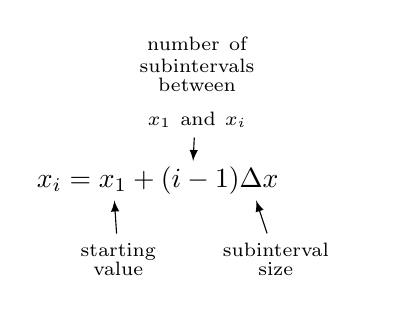
\begin{tikzpicture}[>=latex]
%\draw [thin,step=1cm] (0,0) grid  (3,3);
\draw (1.5,1) node {$\displaystyle x_i = x_1 + (i-1)\Delta x$};

\draw [{\colorone}] (1,0) node [text width=32pt,align=center] (a) {\scriptsize \centering starting\\[-5pt] value};
\draw [{\colorone},->] (a) -- (.95,.75);

\draw [{\colorone}] (2,2.25) node [text width=60pt,align=center] (b) {\scriptsize \centering number of subintervals\\[-5pt] between $x_1$ and $x_i$};
\draw [{\colorone},->] (b) -- (1.95,1.25);

\draw [{\colorone}] (3,0) node [text width=60pt,align=center] (c) {\scriptsize \centering subinterval\\[-5pt] size};
\draw [{\colorone},->] (c) -- (2.75,.75);


\end{tikzpicture}